\chapter{Segment trees revisited}

\index{segment tree}

A segment tree is a versatile data structure that can
be used to solve a large number of algorithm problems.
However, there are many topics related to segment trees
that have not been touched yet. Therefore, it is time
to discuss some more advanced variants of segment trees.

So far, we have implemented the operations
of a segment tree by walking \emph{from bottom to top}
in the tree.
For example, we have calculated
range sums as follows (Chapter 9.3):

\begin{lstlisting}
int sum(int a, int b) {
    a += n; b += n;
    int s = 0;
    while (a <= b) {
        if (a%2 == 1) s += tree[a++];
        if (b%2 == 0) s += tree[b--];
        a /= 2; b /= 2;
    }
    return s;
}
\end{lstlisting}

However, in more advanced segment trees,
it is often necessary to implement the operations
in another way, \emph{from top to bottom}.
Using this approach, the function becomes as follows:
\begin{lstlisting}
int sum(int a, int b, int k, int x, int y) {
    if (b < x || a > y) return 0;
    if (a <= x && y <= b) return tree[k];
    int d = (x+y)/2;
    return sum(a,b,2*k,x,d) + sum(a,b,2*k+1,d+1,y);
}
\end{lstlisting}

Now we can calculate any value of $\texttt{sum}_q(a,b)$
(the sum of array values in range $[a,b]$) as follows:
\begin{lstlisting}
int s = sum(a, b, 1, 0, n-1);
\end{lstlisting}

The parameter $k$ indicates the current position
in \texttt{tree}.
Initially $k$ equals 1, because we begin
at the root of the tree.
The range $[x,y]$ corresponds to $k$
and is initially $[0,n-1]$.
When calculating the sum,
if $[x,y]$ is outside $[a,b]$,
the sum is 0,
and if $[x,y]$ is completely inside $[a,b]$,
the sum can be found in \texttt{tree}.
If $[x,y]$ is partially inside $[a,b]$,
the search continues recursively to the
left and right half of $[x,y]$.
The left half is $[x,d]$
and the right half is $[d+1,y]$
where $d=\lfloor \frac{x+y}{2} \rfloor$.

The following picture shows how the search proceeds
when calculating the value of $\texttt{sum}_q(a,b)$.
The gray nodes indicate nodes where the recursion
stops and the sum can be found in \texttt{tree}.

\begin{center}
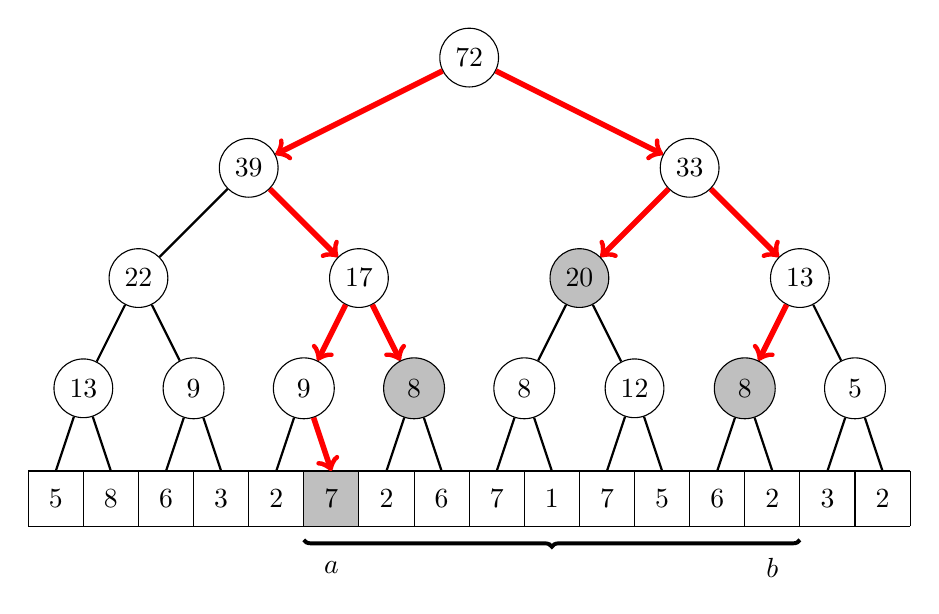
\begin{tikzpicture}[scale=0.7]
\fill[color=gray!50] (5,0) rectangle (6,1);
\draw (0,0) grid (16,1);

\node[anchor=center] at (0.5, 0.5) {5};
\node[anchor=center] at (1.5, 0.5) {8};
\node[anchor=center] at (2.5, 0.5) {6};
\node[anchor=center] at (3.5, 0.5) {3};
\node[anchor=center] at (4.5, 0.5) {2};
\node[anchor=center] at (5.5, 0.5) {7};
\node[anchor=center] at (6.5, 0.5) {2};
\node[anchor=center] at (7.5, 0.5) {6};
\node[anchor=center] at (8.5, 0.5) {7};
\node[anchor=center] at (9.5, 0.5) {1};
\node[anchor=center] at (10.5, 0.5) {7};
\node[anchor=center] at (11.5, 0.5) {5};
\node[anchor=center] at (12.5, 0.5) {6};
\node[anchor=center] at (13.5, 0.5) {2};
\node[anchor=center] at (14.5, 0.5) {3};
\node[anchor=center] at (15.5, 0.5) {2};

%\node[anchor=center] at (1,2.5) {13};

\node[draw, circle] (a) at (1,2.5) {13};
\path[draw,thick,-] (a) -- (0.5,1);
\path[draw,thick,-] (a) -- (1.5,1);
\node[draw, circle,minimum size=22pt] (b) at (3,2.5) {9};
\path[draw,thick,-] (b) -- (2.5,1);
\path[draw,thick,-] (b) -- (3.5,1);
\node[draw, circle,minimum size=22pt] (c) at (5,2.5) {9};
\path[draw,thick,-] (c) -- (4.5,1);
\path[draw,thick,-] (c) -- (5.5,1);
\node[draw, circle,fill=gray!50,minimum size=22pt] (d) at (7,2.5) {8};
\path[draw,thick,-] (d) -- (6.5,1);
\path[draw,thick,-] (d) -- (7.5,1);
\node[draw, circle,minimum size=22pt] (e) at (9,2.5) {8};
\path[draw,thick,-] (e) -- (8.5,1);
\path[draw,thick,-] (e) -- (9.5,1);
\node[draw, circle] (f) at (11,2.5) {12};
\path[draw,thick,-] (f) -- (10.5,1);
\path[draw,thick,-] (f) -- (11.5,1);
\node[draw, circle,fill=gray!50,minimum size=22pt] (g) at (13,2.5) {8};
\path[draw,thick,-] (g) -- (12.5,1);
\path[draw,thick,-] (g) -- (13.5,1);
\node[draw, circle,minimum size=22pt] (h) at (15,2.5) {5};
\path[draw,thick,-] (h) -- (14.5,1);
\path[draw,thick,-] (h) -- (15.5,1);

\node[draw, circle] (i) at (2,4.5) {22};
\path[draw,thick,-] (i) -- (a);
\path[draw,thick,-] (i) -- (b);
\node[draw, circle] (j) at (6,4.5) {17};
\path[draw,thick,-] (j) -- (c);
\path[draw,thick,-] (j) -- (d);
\node[draw, circle,fill=gray!50] (k) at (10,4.5) {20};
\path[draw,thick,-] (k) -- (e);
\path[draw,thick,-] (k) -- (f);
\node[draw, circle] (l) at (14,4.5) {13};
\path[draw,thick,-] (l) -- (g);
\path[draw,thick,-] (l) -- (h);

\node[draw, circle] (m) at (4,6.5) {39};
\path[draw,thick,-] (m) -- (i);
\path[draw,thick,-] (m) -- (j);
\node[draw, circle] (n) at (12,6.5) {33};
\path[draw,thick,-] (n) -- (k);
\path[draw,thick,-] (n) -- (l);

\node[draw, circle] (o) at (8,8.5) {72};
\path[draw,thick,-] (o) -- (m);
\path[draw,thick,-] (o) -- (n);

\path[draw=red,thick,->,line width=2pt] (o) -- (m);
\path[draw=red,thick,->,line width=2pt] (o) -- (n);

\path[draw=red,thick,->,line width=2pt] (m) -- (j);
\path[draw=red,thick,->,line width=2pt] (j) -- (c);
\path[draw=red,thick,->,line width=2pt] (j) -- (d);
\path[draw=red,thick,->,line width=2pt] (c) -- (5.5,1);

\path[draw=red,thick,->,line width=2pt] (n) -- (k);
\path[draw=red,thick,->,line width=2pt] (n) -- (l);

\path[draw=red,thick,->,line width=2pt] (l) -- (g);

\draw [decoration={brace}, decorate, line width=0.5mm] (14,-0.25) -- (5,-0.25);

\node at (5.5,-0.75) {$a$};
\node at (13.5,-0.75) {$b$};
\end{tikzpicture}
\end{center}

Also in this implementation,
operations take $O(\log n)$ time,
because the total number of visited nodes is $O(\log n)$.

\section{Lazy propagation}

\index{lazy propagation}
\index{lazy segment tree}

Using \key{lazy propagation}, we can build
a segment tree that supports \emph{both} range updates
and range queries in $O(\log n)$ time.
The idea is to perform updates and queries
from top to bottom and perform updates
\emph{lazily} so that they are propagated
down the tree only when it is necessary.

In a lazy segment tree, nodes contain two types of
information.
Like in an ordinary segment tree,
each node contains the sum or some other value
related to the corresponding subarray.
In addition, the node may contain information
related to lazy updates, which has not been
propagated to its children.

There are two types of range updates:
each array value in the range is either
\emph{increased} by some value
or \emph{assigned} some value.
Both operations can be implemented using
similar ideas, and it is even possible to construct
a tree that supports both operations at the same time.

\subsubsection{Lazy segment trees}

Let us consider an example where our goal is to
construct a segment tree that supports
two operations: increasing each value in
$[a,b]$ by a constant and calculating the sum of
values in $[a,b]$.

We will construct a tree where each node
has two values $s/z$:
$s$ denotes the sum of values in the range,
and $z$ denotes the value of a lazy update,
which means that all values in the range
should be increased by $z$.
In the following tree, $z=0$ in all nodes,
so there are no ongoing lazy updates.
\begin{center}
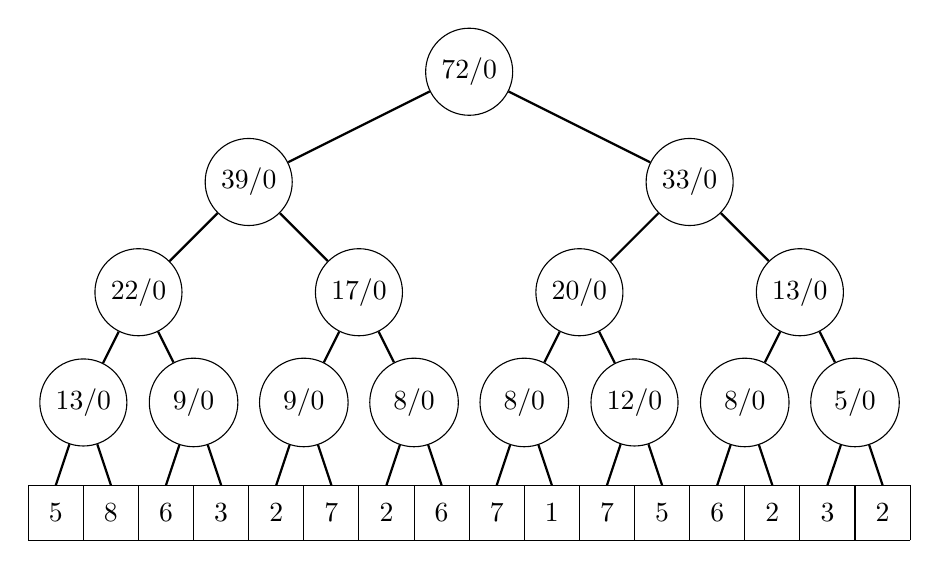
\begin{tikzpicture}[scale=0.7]
\draw (0,0) grid (16,1);

\node[anchor=center] at (0.5, 0.5) {5};
\node[anchor=center] at (1.5, 0.5) {8};
\node[anchor=center] at (2.5, 0.5) {6};
\node[anchor=center] at (3.5, 0.5) {3};
\node[anchor=center] at (4.5, 0.5) {2};
\node[anchor=center] at (5.5, 0.5) {7};
\node[anchor=center] at (6.5, 0.5) {2};
\node[anchor=center] at (7.5, 0.5) {6};
\node[anchor=center] at (8.5, 0.5) {7};
\node[anchor=center] at (9.5, 0.5) {1};
\node[anchor=center] at (10.5, 0.5) {7};
\node[anchor=center] at (11.5, 0.5) {5};
\node[anchor=center] at (12.5, 0.5) {6};
\node[anchor=center] at (13.5, 0.5) {2};
\node[anchor=center] at (14.5, 0.5) {3};
\node[anchor=center] at (15.5, 0.5) {2};

\node[draw, circle] (a) at (1,2.5) {13/0};
\path[draw,thick,-] (a) -- (0.5,1);
\path[draw,thick,-] (a) -- (1.5,1);
\node[draw, circle,minimum size=32pt] (b) at (3,2.5) {9/0};
\path[draw,thick,-] (b) -- (2.5,1);
\path[draw,thick,-] (b) -- (3.5,1);
\node[draw, circle,minimum size=32pt] (c) at (5,2.5) {9/0};
\path[draw,thick,-] (c) -- (4.5,1);
\path[draw,thick,-] (c) -- (5.5,1);
\node[draw, circle,minimum size=32pt] (d) at (7,2.5) {8/0};
\path[draw,thick,-] (d) -- (6.5,1);
\path[draw,thick,-] (d) -- (7.5,1);
\node[draw, circle,minimum size=32pt] (e) at (9,2.5) {8/0};
\path[draw,thick,-] (e) -- (8.5,1);
\path[draw,thick,-] (e) -- (9.5,1);
\node[draw, circle] (f) at (11,2.5) {12/0};
\path[draw,thick,-] (f) -- (10.5,1);
\path[draw,thick,-] (f) -- (11.5,1);
\node[draw, circle,minimum size=32pt] (g) at (13,2.5) {8/0};
\path[draw,thick,-] (g) -- (12.5,1);
\path[draw,thick,-] (g) -- (13.5,1);
\node[draw, circle,minimum size=32pt] (h) at (15,2.5) {5/0};
\path[draw,thick,-] (h) -- (14.5,1);
\path[draw,thick,-] (h) -- (15.5,1);

\node[draw, circle] (i) at (2,4.5) {22/0};
\path[draw,thick,-] (i) -- (a);
\path[draw,thick,-] (i) -- (b);
\node[draw, circle] (j) at (6,4.5) {17/0};
\path[draw,thick,-] (j) -- (c);
\path[draw,thick,-] (j) -- (d);
\node[draw, circle] (k) at (10,4.5) {20/0};
\path[draw,thick,-] (k) -- (e);
\path[draw,thick,-] (k) -- (f);
\node[draw, circle] (l) at (14,4.5) {13/0};
\path[draw,thick,-] (l) -- (g);
\path[draw,thick,-] (l) -- (h);

\node[draw, circle] (m) at (4,6.5) {39/0};
\path[draw,thick,-] (m) -- (i);
\path[draw,thick,-] (m) -- (j);
\node[draw, circle] (n) at (12,6.5) {33/0};
\path[draw,thick,-] (n) -- (k);
\path[draw,thick,-] (n) -- (l);

\node[draw, circle] (o) at (8,8.5) {72/0};
\path[draw,thick,-] (o) -- (m);
\path[draw,thick,-] (o) -- (n);
\end{tikzpicture}
\end{center}

When the elements in $[a,b]$ are increased by $u$,
we walk from the root towards the leaves
and modify the nodes of the tree as follows:
If the range $[x,y]$ of a node is
completely inside $[a,b]$,
we increase the $z$ value of the node by $u$ and stop.
If $[x,y]$ only partially belongs to $[a,b]$,
we increase the $s$ value of the node by $hu$,
where $h$ is the size of the intersection of $[a,b]$
and $[x,y]$, and continue our walk recursively in the tree.

For example, the following picture shows the tree after
increasing the elements in $[a,b]$ by 2:
\begin{center}
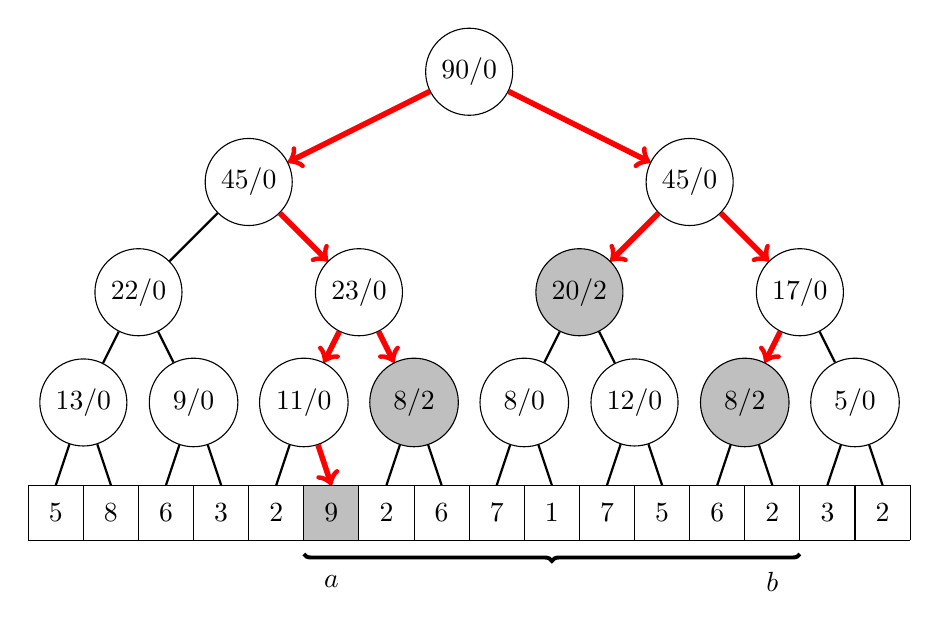
\begin{tikzpicture}[scale=0.7]
\fill[color=gray!50] (5,0) rectangle (6,1);
\draw (0,0) grid (16,1);

\node[anchor=center] at (0.5, 0.5) {5};
\node[anchor=center] at (1.5, 0.5) {8};
\node[anchor=center] at (2.5, 0.5) {6};
\node[anchor=center] at (3.5, 0.5) {3};
\node[anchor=center] at (4.5, 0.5) {2};
\node[anchor=center] at (5.5, 0.5) {9};
\node[anchor=center] at (6.5, 0.5) {2};
\node[anchor=center] at (7.5, 0.5) {6};
\node[anchor=center] at (8.5, 0.5) {7};
\node[anchor=center] at (9.5, 0.5) {1};
\node[anchor=center] at (10.5, 0.5) {7};
\node[anchor=center] at (11.5, 0.5) {5};
\node[anchor=center] at (12.5, 0.5) {6};
\node[anchor=center] at (13.5, 0.5) {2};
\node[anchor=center] at (14.5, 0.5) {3};
\node[anchor=center] at (15.5, 0.5) {2};

\node[draw, circle] (a) at (1,2.5) {13/0};
\path[draw,thick,-] (a) -- (0.5,1);
\path[draw,thick,-] (a) -- (1.5,1);
\node[draw, circle,minimum size=32pt] (b) at (3,2.5) {9/0};
\path[draw,thick,-] (b) -- (2.5,1);
\path[draw,thick,-] (b) -- (3.5,1);
\node[draw, circle,minimum size=32pt] (c) at (5,2.5) {11/0};
\path[draw,thick,-] (c) -- (4.5,1);
\path[draw,thick,-] (c) -- (5.5,1);
\node[draw, circle,fill=gray!50,minimum size=32pt] (d) at (7,2.5) {8/2};
\path[draw,thick,-] (d) -- (6.5,1);
\path[draw,thick,-] (d) -- (7.5,1);
\node[draw, circle,minimum size=32pt] (e) at (9,2.5) {8/0};
\path[draw,thick,-] (e) -- (8.5,1);
\path[draw,thick,-] (e) -- (9.5,1);
\node[draw, circle] (f) at (11,2.5) {12/0};
\path[draw,thick,-] (f) -- (10.5,1);
\path[draw,thick,-] (f) -- (11.5,1);
\node[draw, circle,fill=gray!50,minimum size=32pt] (g) at (13,2.5) {8/2};
\path[draw,thick,-] (g) -- (12.5,1);
\path[draw,thick,-] (g) -- (13.5,1);
\node[draw, circle,minimum size=32pt] (h) at (15,2.5) {5/0};
\path[draw,thick,-] (h) -- (14.5,1);
\path[draw,thick,-] (h) -- (15.5,1);

\node[draw, circle] (i) at (2,4.5) {22/0};
\path[draw,thick,-] (i) -- (a);
\path[draw,thick,-] (i) -- (b);
\node[draw, circle] (j) at (6,4.5) {23/0};
\path[draw,thick,-] (j) -- (c);
\path[draw,thick,-] (j) -- (d);
\node[draw, circle,fill=gray!50] (k) at (10,4.5) {20/2};
\path[draw,thick,-] (k) -- (e);
\path[draw,thick,-] (k) -- (f);
\node[draw, circle] (l) at (14,4.5) {17/0};
\path[draw,thick,-] (l) -- (g);
\path[draw,thick,-] (l) -- (h);

\node[draw, circle] (m) at (4,6.5) {45/0};
\path[draw,thick,-] (m) -- (i);
\path[draw,thick,-] (m) -- (j);
\node[draw, circle] (n) at (12,6.5) {45/0};
\path[draw,thick,-] (n) -- (k);
\path[draw,thick,-] (n) -- (l);

\node[draw, circle] (o) at (8,8.5) {90/0};
\path[draw,thick,-] (o) -- (m);
\path[draw,thick,-] (o) -- (n);

\path[draw=red,thick,->,line width=2pt] (o) -- (m);
\path[draw=red,thick,->,line width=2pt] (o) -- (n);

\path[draw=red,thick,->,line width=2pt] (m) -- (j);
\path[draw=red,thick,->,line width=2pt] (j) -- (c);
\path[draw=red,thick,->,line width=2pt] (j) -- (d);
\path[draw=red,thick,->,line width=2pt] (c) -- (5.5,1);

\path[draw=red,thick,->,line width=2pt] (n) -- (k);
\path[draw=red,thick,->,line width=2pt] (n) -- (l);

\path[draw=red,thick,->,line width=2pt] (l) -- (g);

\draw [decoration={brace}, decorate, line width=0.5mm] (14,-0.25) -- (5,-0.25);

\node at (5.5,-0.75) {$a$};
\node at (13.5,-0.75) {$b$};
\end{tikzpicture}
\end{center}

We also calculate the sum of elements in a range $[a,b]$
by walking in the tree from top to bottom.
If the range $[x,y]$ of a node completely belongs
to $[a,b]$, we add the $s$ value of the node to the sum.
Otherwise, we continue the search recursively
downwards in the tree.

Both in updates and queries,
the value of a lazy update is always propagated
to the children of the node
before processing the node.
The idea is that updates will be propagated
downwards only when it is necessary,
which guarantees that the operations are always efficient.

The following picture shows how the tree changes
when we calculate the value of $\texttt{sum}_a(a,b)$.
The rectangle shows the nodes whose values change,
because a lazy update is propagated downwards.

\begin{center}
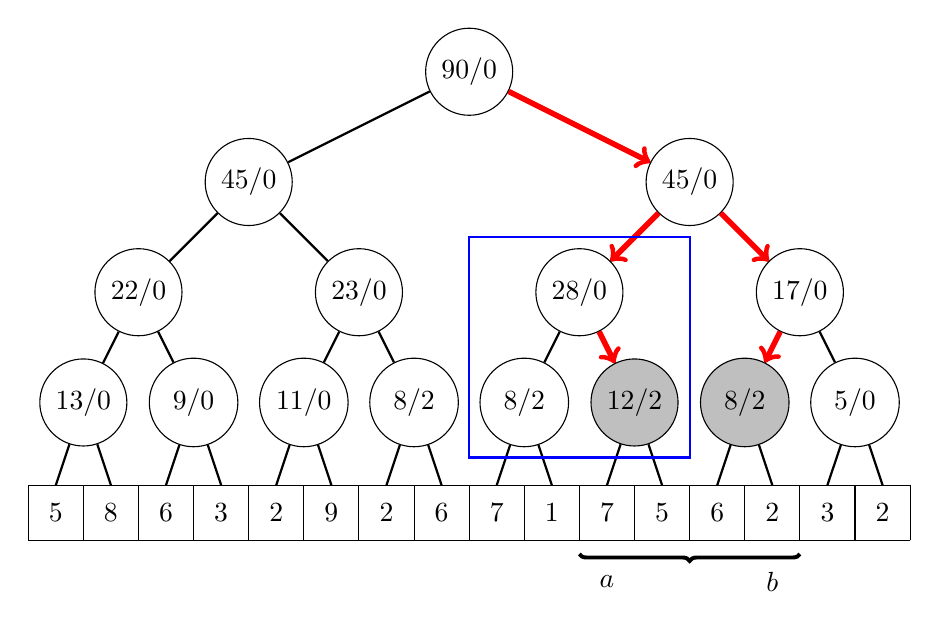
\begin{tikzpicture}[scale=0.7]
\draw (0,0) grid (16,1);

\node[anchor=center] at (0.5, 0.5) {5};
\node[anchor=center] at (1.5, 0.5) {8};
\node[anchor=center] at (2.5, 0.5) {6};
\node[anchor=center] at (3.5, 0.5) {3};
\node[anchor=center] at (4.5, 0.5) {2};
\node[anchor=center] at (5.5, 0.5) {9};
\node[anchor=center] at (6.5, 0.5) {2};
\node[anchor=center] at (7.5, 0.5) {6};
\node[anchor=center] at (8.5, 0.5) {7};
\node[anchor=center] at (9.5, 0.5) {1};
\node[anchor=center] at (10.5, 0.5) {7};
\node[anchor=center] at (11.5, 0.5) {5};
\node[anchor=center] at (12.5, 0.5) {6};
\node[anchor=center] at (13.5, 0.5) {2};
\node[anchor=center] at (14.5, 0.5) {3};
\node[anchor=center] at (15.5, 0.5) {2};

\node[draw, circle] (a) at (1,2.5) {13/0};
\path[draw,thick,-] (a) -- (0.5,1);
\path[draw,thick,-] (a) -- (1.5,1);
\node[draw, circle,minimum size=32pt] (b) at (3,2.5) {9/0};
\path[draw,thick,-] (b) -- (2.5,1);
\path[draw,thick,-] (b) -- (3.5,1);
\node[draw, circle,minimum size=32pt] (c) at (5,2.5) {11/0};
\path[draw,thick,-] (c) -- (4.5,1);
\path[draw,thick,-] (c) -- (5.5,1);
\node[draw, circle,minimum size=32pt] (d) at (7,2.5) {8/2};
\path[draw,thick,-] (d) -- (6.5,1);
\path[draw,thick,-] (d) -- (7.5,1);
\node[draw, circle,minimum size=32pt] (e) at (9,2.5) {8/2};
\path[draw,thick,-] (e) -- (8.5,1);
\path[draw,thick,-] (e) -- (9.5,1);
\node[draw, circle,fill=gray!50,] (f) at (11,2.5) {12/2};
\path[draw,thick,-] (f) -- (10.5,1);
\path[draw,thick,-] (f) -- (11.5,1);
\node[draw, circle,fill=gray!50,minimum size=32pt] (g) at (13,2.5) {8/2};
\path[draw,thick,-] (g) -- (12.5,1);
\path[draw,thick,-] (g) -- (13.5,1);
\node[draw, circle,minimum size=32pt] (h) at (15,2.5) {5/0};
\path[draw,thick,-] (h) -- (14.5,1);
\path[draw,thick,-] (h) -- (15.5,1);

\node[draw, circle] (i) at (2,4.5) {22/0};
\path[draw,thick,-] (i) -- (a);
\path[draw,thick,-] (i) -- (b);
\node[draw, circle] (j) at (6,4.5) {23/0};
\path[draw,thick,-] (j) -- (c);
\path[draw,thick,-] (j) -- (d);
\node[draw, circle] (k) at (10,4.5) {28/0};
\path[draw,thick,-] (k) -- (e);
\path[draw,thick,-] (k) -- (f);
\node[draw, circle] (l) at (14,4.5) {17/0};
\path[draw,thick,-] (l) -- (g);
\path[draw,thick,-] (l) -- (h);

\node[draw, circle] (m) at (4,6.5) {45/0};
\path[draw,thick,-] (m) -- (i);
\path[draw,thick,-] (m) -- (j);
\node[draw, circle] (n) at (12,6.5) {45/0};
\path[draw,thick,-] (n) -- (k);
\path[draw,thick,-] (n) -- (l);

\node[draw, circle] (o) at (8,8.5) {90/0};
\path[draw,thick,-] (o) -- (m);
\path[draw,thick,-] (o) -- (n);

\path[draw=red,thick,->,line width=2pt] (o) -- (n);

\path[draw=red,thick,->,line width=2pt] (n) -- (k);
\path[draw=red,thick,->,line width=2pt] (n) -- (l);

\path[draw=red,thick,->,line width=2pt] (k) -- (f);
\path[draw=red,thick,->,line width=2pt] (l) -- (g);

\draw [decoration={brace}, decorate, line width=0.5mm] (14,-0.25) -- (10,-0.25);

\draw[color=blue,thick] (8,1.5) rectangle (12,5.5);

\node at (10.5,-0.75) {$a$};
\node at (13.5,-0.75) {$b$};
\end{tikzpicture}
\end{center}

Note that sometimes it is needed to combine lazy updates.
This happens when a node that already has a lazy update
is assigned another lazy update.
When calculating sums, it is easy to combine lazy updates,
because the combination of updates $z_1$ and $z_2$
corresponds to an update $z_1+z_2$.

\subsubsection{Polynomial updates}

Lazy updates can be generalized so that it is
possible to update ranges using polynomials of the form
\[p(u) = t_k u^k + t_{k-1} u^{k-1} + \cdots + t_0.\]

In this case, the update for a value
at position $i$ in $[a,b]$ is $p(i-a)$.
For example, adding the polynomial $p(u)=u+1$
to $[a,b]$ means that the value at position $a$
increases by 1, the value at position $a+1$
increases by 2, and so on.

To support polynomial updates,
each node is assigned $k+2$ values,
where $k$ equals the degree of the polynomial.
The value $s$ is the sum of the elements in the range,
and the values $z_0,z_1,\ldots,z_k$ are the coefficients
of a polynomial that corresponds to a lazy update.

Now, the sum of values in a range $[x,y]$ equals
\[s+\sum_{u=0}^{y-x} z_k u^k + z_{k-1} u^{k-1} + \cdots + z_0.\]

The value of such a sum
can be efficiently calculated using sum formulas.
For example, the term $z_0$ corresponds to the sum
$(y-x+1)z_0$, and the term $z_1 u$ corresponds to the sum
\[z_1(0+1+\cdots+y-x) = z_1 \frac{(y-x)(y-x+1)}{2} .\]

When propagating an update in the tree,
the indices of $p(u)$ change,
because in each range $[x,y]$,
the values are
calculated for $u=0,1,\ldots,y-x$.
However, this is not a problem, because
$p'(u)=p(u+h)$ is a polynomial
of equal degree as $p(u)$.
For example, if $p(u)=t_2 u^2+t_1 u-t_0$, then
\[p'(u)=t_2(u+h)^2+t_1(u+h)-t_0=t_2 u^2 + (2ht_2+t_1)u+t_2h^2+t_1h-t_0.\]

\section{Dynamic trees}

\index{dynamic segment tree}

An ordinary segment tree is static,
which means that each node has a fixed position
in the array and the tree requires
a fixed amount of memory.
In a \key{dynamic segment tree},
memory is allocated only for nodes that
are actually accessed during the algorithm,
which can save a large amount of memory.

The nodes of a dynamic tree can be represented as structs:
\begin{lstlisting}
struct node {
    int value;
    int x, y;
    node *left, *right;
    node(int v, int x, int y) : value(v), x(x), y(y) {}
};
\end{lstlisting}
Here \texttt{value} is the value of the node,
$[\texttt{x},\texttt{y}]$ is the corresponding range,
and \texttt{left} and \texttt{right} point to the left
and right subtree.

After this, nodes can be created as follows:
\begin{lstlisting}
// create new node
node *x = new node(0, 0, 15);
// change value
x->value = 5;
\end{lstlisting}

\subsubsection{Sparse segment trees}

\index{sparse segment tree}

A dynamic segment tree is useful when
the underlying array is \emph{sparse},
i.e., the range $[0,n-1]$
of allowed indices is large,
but most array values are zeros.
While an ordinary segment tree uses $O(n)$ memory,
a dynamic segment tree only uses $O(k \log n)$ memory,
where $k$ is the number of operations performed.

A \key{sparse segment tree} initially has
only one node $[0,n-1]$ whose value is zero,
which means that every array value is zero.
After updates, new nodes are dynamically added
to the tree.
For example, if $n=16$ and the elements
in positions 3 and 10 have been modified,
the tree contains the following nodes:
\begin{center}
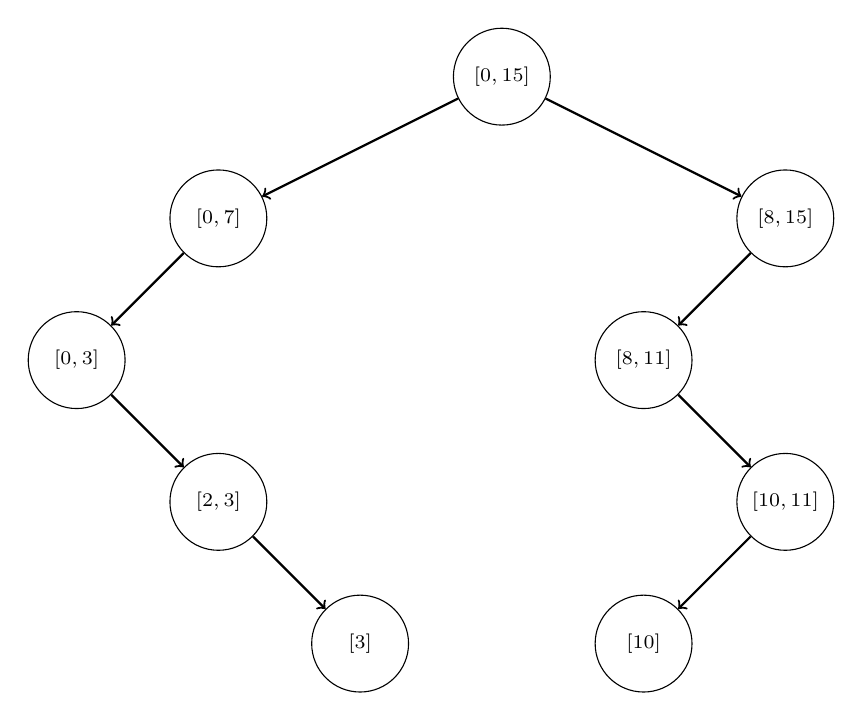
\begin{tikzpicture}[scale=0.9]
\scriptsize
\node[draw, circle,minimum size=35pt] (1) at (0,0) {$[0,15]$};
\node[draw, circle,minimum size=35pt] (2) at (-4,-2) {$[0,7]$};
\node[draw, circle,minimum size=35pt] (3) at (-6,-4) {$[0,3]$};
\node[draw, circle,minimum size=35pt] (4) at (-4,-6) {$[2,3]$};
\node[draw, circle,minimum size=35pt] (5) at (-2,-8) {$[3]$};
\node[draw, circle,minimum size=35pt] (6) at (4,-2) {$[8,15]$};
\node[draw, circle,minimum size=35pt] (7) at (2,-4) {$[8,11]$};
\node[draw, circle,minimum size=35pt] (8) at (4,-6) {$[10,11]$};
\node[draw, circle,minimum size=35pt] (9) at (2,-8) {$[10]$};

\path[draw,thick,->] (1) -- (2);
\path[draw,thick,->] (2) -- (3);
\path[draw,thick,->] (3) -- (4);
\path[draw,thick,->] (4) -- (5);

\path[draw,thick,->] (1) -- (6);
\path[draw,thick,->] (6) -- (7);
\path[draw,thick,->] (7) -- (8);
\path[draw,thick,->] (8) -- (9);
\end{tikzpicture}
\end{center}

Any path from the root node to a leaf contains
$O(\log n)$ nodes,
so each operation adds at most $O(\log n)$
new nodes to the tree.
Thus, after $k$ operations, the tree contains
at most $O(k \log n)$ nodes.

Note that if we know all elements to be updated
at the beginning of the algorithm,
a dynamic segment tree is not necessary,
because we can use an ordinary segment tree with
index compression (Chapter 9.4).
However, this is not possible when the indices
are generated during the algorithm.

\subsubsection{Persistent segment trees}

\index{persistent segment tree}

Using a dynamic implementation,
it is also possible to create a
\key{persistent segment tree} that stores
the \emph{modification history} of the tree.
In such an implementation, we can
efficiently access
all versions of the tree that have
existed during the algorithm.

When the modification history is available,
we can perform queries in any previous tree
like in an ordinary segment tree, because the
full structure of each tree is stored.
We can also create new trees based on previous
trees and modify them independently.

Consider the following sequence of updates,
where red nodes change
and other nodes remain the same:

\begin{center}
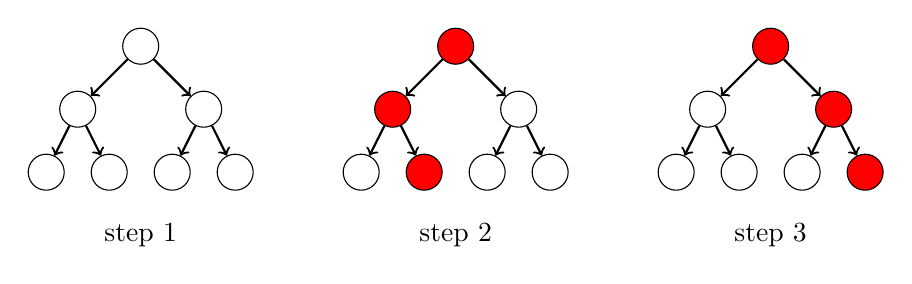
\begin{tikzpicture}[scale=0.8]
\node[draw, circle,minimum size=13pt] (1a) at (3,0) {};
\node[draw, circle,minimum size=13pt] (2a) at (2,-1) {};
\node[draw, circle,minimum size=13pt] (3a) at (4,-1) {};
\node[draw, circle,minimum size=13pt] (4a) at (1.5,-2) {};
\node[draw, circle,minimum size=13pt] (5a) at (2.5,-2) {};
\node[draw, circle,minimum size=13pt] (6a) at (3.5,-2) {};
\node[draw, circle,minimum size=13pt] (7a) at (4.5,-2) {};
\path[draw,thick,->] (1a) -- (2a);
\path[draw,thick,->] (1a) -- (3a);
\path[draw,thick,->] (2a) -- (4a);
\path[draw,thick,->] (2a) -- (5a);
\path[draw,thick,->] (3a) -- (6a);
\path[draw,thick,->] (3a) -- (7a);

\node[draw, circle,minimum size=13pt,fill=red] (1b) at (3+5,0) {};
\node[draw, circle,minimum size=13pt,fill=red] (2b) at (2+5,-1) {};
\node[draw, circle,minimum size=13pt] (3b) at (4+5,-1) {};
\node[draw, circle,minimum size=13pt] (4b) at (1.5+5,-2) {};
\node[draw, circle,minimum size=13pt,fill=red] (5b) at (2.5+5,-2) {};
\node[draw, circle,minimum size=13pt] (6b) at (3.5+5,-2) {};
\node[draw, circle,minimum size=13pt] (7b) at (4.5+5,-2) {};
\path[draw,thick,->] (1b) -- (2b);
\path[draw,thick,->] (1b) -- (3b);
\path[draw,thick,->] (2b) -- (4b);
\path[draw,thick,->] (2b) -- (5b);
\path[draw,thick,->] (3b) -- (6b);
\path[draw,thick,->] (3b) -- (7b);

\node[draw, circle,minimum size=13pt,fill=red] (1c) at (3+10,0) {};
\node[draw, circle,minimum size=13pt] (2c) at (2+10,-1) {};
\node[draw, circle,minimum size=13pt,fill=red] (3c) at (4+10,-1) {};
\node[draw, circle,minimum size=13pt] (4c) at (1.5+10,-2) {};
\node[draw, circle,minimum size=13pt] (5c) at (2.5+10,-2) {};
\node[draw, circle,minimum size=13pt] (6c) at (3.5+10,-2) {};
\node[draw, circle,minimum size=13pt,fill=red] (7c) at (4.5+10,-2) {};
\path[draw,thick,->] (1c) -- (2c);
\path[draw,thick,->] (1c) -- (3c);
\path[draw,thick,->] (2c) -- (4c);
\path[draw,thick,->] (2c) -- (5c);
\path[draw,thick,->] (3c) -- (6c);
\path[draw,thick,->] (3c) -- (7c);

\node at (3,-3) {step 1};
\node at (3+5,-3) {step 2};
\node at (3+10,-3) {step 3};
\end{tikzpicture}
\end{center}
After each update, most nodes of the tree
remain the same,
so an efficient way to store the modification history
is to represent each tree in the history as a combination
of new nodes and subtrees of previous trees.
In this example, the modification history can be
stored as follows:
\begin{center}
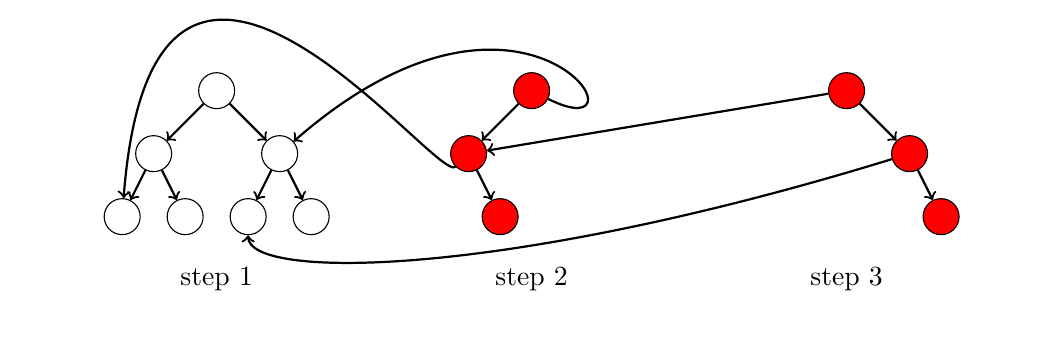
\begin{tikzpicture}[scale=0.8]
\path[use as bounding box] (0, 1) rectangle (16, -3.5);

\node[draw, circle,minimum size=13pt] (1a) at (3,0) {};
\node[draw, circle,minimum size=13pt] (2a) at (2,-1) {};
\node[draw, circle,minimum size=13pt] (3a) at (4,-1) {};
\node[draw, circle,minimum size=13pt] (4a) at (1.5,-2) {};
\node[draw, circle,minimum size=13pt] (5a) at (2.5,-2) {};
\node[draw, circle,minimum size=13pt] (6a) at (3.5,-2) {};
\node[draw, circle,minimum size=13pt] (7a) at (4.5,-2) {};
\path[draw,thick,->] (1a) -- (2a);
\path[draw,thick,->] (1a) -- (3a);
\path[draw,thick,->] (2a) -- (4a);
\path[draw,thick,->] (2a) -- (5a);
\path[draw,thick,->] (3a) -- (6a);
\path[draw,thick,->] (3a) -- (7a);

\node[draw, circle,minimum size=13pt,fill=red] (1b) at (3+5,0) {};
\node[draw, circle,minimum size=13pt,fill=red] (2b) at (2+5,-1) {};
\node[draw, circle,minimum size=13pt,fill=red] (5b) at (2.5+5,-2) {};
\path[draw,thick,->] (1b) -- (2b);

\draw[thick,->] (1b) .. controls (3+5+2,0-1) and (3+5,2.5) .. (3a);

\draw[thick,->] (2b) .. controls (2+5-0.5,-1-0.5) and (2,4.5) .. (4a);


\path[draw,thick,->] (2b) -- (5b);

\node[draw, circle,minimum size=13pt,fill=red] (1c) at (3+10,0) {};
\node[draw, circle,minimum size=13pt,fill=red] (3c) at (4+10,-1) {};
\node[draw, circle,minimum size=13pt,fill=red] (7c) at (4.5+10,-2) {};
\path[draw,thick,->] (1c) -- (2b);
\path[draw,thick,->] (1c) -- (3c);

\draw[thick,->] (3c) .. controls (2.5+5,-3) and (3.5,-3) .. (6a);

\path[draw,thick,->] (3c) -- (7c);

\node at (3,-3) {step 1};
\node at (3+5,-3) {step 2};
\node at (3+10,-3) {step 3};
\end{tikzpicture}
\end{center}

The structure of each previous tree can be
reconstructed by following the pointers
starting at the corresponding root node.
Since each operation
adds only $O(\log n)$ new nodes to the tree,
it is possible to store the full modification history of the tree.

\section{Data structures}

Instead of single values, nodes in a segment tree
can also contain \emph{data structures} that maintain information
about the corresponding ranges.
In such a tree, the operations take
$O(f(n) \log n)$ time, where $f(n)$ is
the time needed for processing a single node during an operation.

As an example, consider a segment tree that
supports queries of the form
''how many times does an element $x$ appear
in the range $[a,b]$?''
For example, the element 1 appears three times
in the following range:

\begin{center}
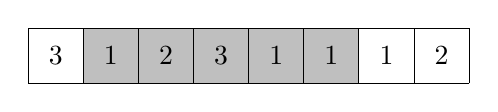
\begin{tikzpicture}[scale=0.7]
\fill[lightgray] (1,0) rectangle (6,1);
\draw (0,0) grid (8,1);

\node[anchor=center] at (0.5, 0.5) {3};
\node[anchor=center] at (1.5, 0.5) {1};
\node[anchor=center] at (2.5, 0.5) {2};
\node[anchor=center] at (3.5, 0.5) {3};
\node[anchor=center] at (4.5, 0.5) {1};
\node[anchor=center] at (5.5, 0.5) {1};
\node[anchor=center] at (6.5, 0.5) {1};
\node[anchor=center] at (7.5, 0.5) {2};
\end{tikzpicture}
\end{center}

To support such queries, we build a segment tree
where each node is assigned a data structure
that can be asked how many times any element $x$
appears in the corresponding range.
Using this tree,
the answer to a query can be calculated
by combining the results from the nodes
that belong to the range.

For example, the following segment tree
corresponds to the above array:
\begin{center}
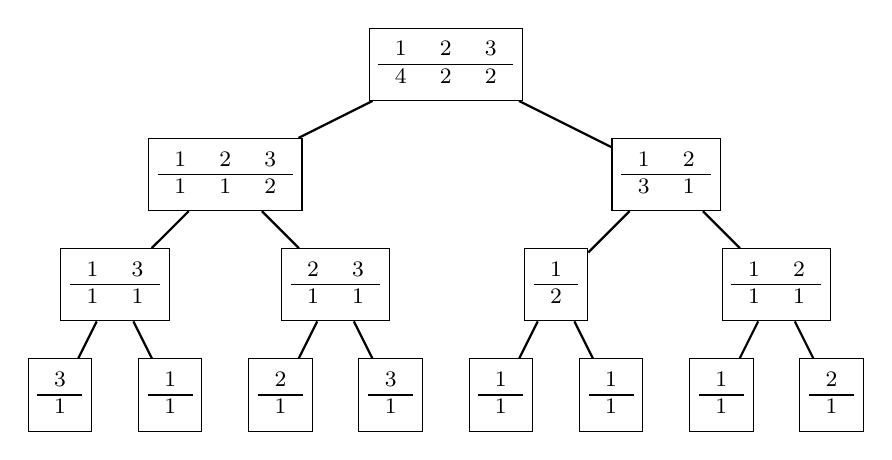
\begin{tikzpicture}[scale=0.7]

\node[draw, rectangle] (a) at (1,2.5)
{
\footnotesize
\begin{tabular}{r}
3 \\
\hline
1 \\
\end{tabular}};
\node[draw, rectangle] (b) at (3,2.5)
{
\footnotesize
\begin{tabular}{r}
1 \\
\hline
1 \\
\end{tabular}};
\node[draw, rectangle] (c) at (5,2.5)
{
\footnotesize
\begin{tabular}{r}
2 \\
\hline
1 \\
\end{tabular}};
\node[draw, rectangle] (d) at (7,2.5)
{
\footnotesize
\begin{tabular}{r}
3 \\
\hline
1 \\
\end{tabular}};
\node[draw, rectangle] (e) at (9,2.5)
{
\footnotesize
\begin{tabular}{r}
1 \\
\hline
1 \\
\end{tabular}};
\node[draw, rectangle] (f) at (11,2.5)
{
\footnotesize
\begin{tabular}{r}
1 \\
\hline
1 \\
\end{tabular}};
\node[draw, rectangle] (g) at (13,2.5)
{
\footnotesize
\begin{tabular}{r}
1 \\
\hline
1 \\
\end{tabular}};
\node[draw, rectangle] (h) at (15,2.5)
{
\footnotesize
\begin{tabular}{r}
2 \\
\hline
1 \\
\end{tabular}};

\node[draw, rectangle] (i) at (2,4.5)
{
\footnotesize
\begin{tabular}{rr}
1 & 3 \\
\hline
1 & 1 \\
\end{tabular}};
\path[draw,thick,-] (i) -- (a);
\path[draw,thick,-] (i) -- (b);
\node[draw, rectangle] (j) at (6,4.5)
{
\footnotesize
\begin{tabular}{rr}
2 & 3 \\
\hline
1 & 1 \\
\end{tabular}};
\path[draw,thick,-] (j) -- (c);
\path[draw,thick,-] (j) -- (d);
\node[draw, rectangle] (k) at (10,4.5)
{
\footnotesize
\begin{tabular}{r}
1 \\
\hline
2 \\
\end{tabular}};
\path[draw,thick,-] (k) -- (e);
\path[draw,thick,-] (k) -- (f);
\node[draw, rectangle] (l) at (14,4.5)
{
\footnotesize
\begin{tabular}{rr}
1 & 2 \\
\hline
1 & 1 \\
\end{tabular}};
\path[draw,thick,-] (l) -- (g);
\path[draw,thick,-] (l) -- (h);

\node[draw, rectangle] (m) at (4,6.5)
{
\footnotesize
\begin{tabular}{rrr}
1 & 2 & 3 \\
\hline
1 & 1 & 2 \\
\end{tabular}};
\path[draw,thick,-] (m) -- (i);
\path[draw,thick,-] (m) -- (j);
\node[draw, rectangle] (n) at (12,6.5)
{
\footnotesize
\begin{tabular}{rr}
1 & 2 \\
\hline
3 & 1 \\
\end{tabular}};
\path[draw,thick,-] (n) -- (k);
\path[draw,thick,-] (n) -- (l);

\node[draw, rectangle] (o) at (8,8.5)
{
\footnotesize
\begin{tabular}{rrr}
1 & 2 & 3 \\
\hline
4 & 2 & 2 \\
\end{tabular}};
\path[draw,thick,-] (o) -- (m);
\path[draw,thick,-] (o) -- (n);
\end{tikzpicture}
\end{center}

We can build the tree so
that each node contains a \texttt{map} structure.
In this case, the time needed for processing each
node is $O(\log n)$, so the total time complexity
of a query is $O(\log^2 n)$.
The tree uses $O(n \log n)$ memory,
because there are $O(\log n)$ levels
and each level contains
$O(n)$ elements.

\section{Two-dimensionality}

\index{two-dimensional segment tree}

A \key{two-dimensional segment tree} supports
queries related to rectangular subarrays
of a two-dimensional array.
Such a tree can be implemented as
nested segment trees: a big tree corresponds to the
rows of the array, and each node contains a small tree
that corresponds to a column.

For example, in the array
\begin{center}
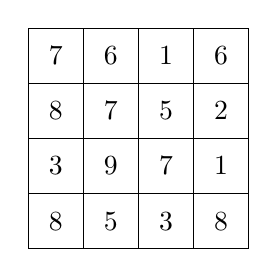
\begin{tikzpicture}[scale=0.7]
\draw (0,0) grid (4,4);

\node[anchor=center] at (0.5, 0.5) {8};
\node[anchor=center] at (1.5, 0.5) {5};
\node[anchor=center] at (2.5, 0.5) {3};
\node[anchor=center] at (3.5, 0.5) {8};

\node[anchor=center] at (0.5, 1.5) {3};
\node[anchor=center] at (1.5, 1.5) {9};
\node[anchor=center] at (2.5, 1.5) {7};
\node[anchor=center] at (3.5, 1.5) {1};

\node[anchor=center] at (0.5, 2.5) {8};
\node[anchor=center] at (1.5, 2.5) {7};
\node[anchor=center] at (2.5, 2.5) {5};
\node[anchor=center] at (3.5, 2.5) {2};

\node[anchor=center] at (0.5, 3.5) {7};
\node[anchor=center] at (1.5, 3.5) {6};
\node[anchor=center] at (2.5, 3.5) {1};
\node[anchor=center] at (3.5, 3.5) {6};
\end{tikzpicture}
\end{center}
the sum of any subarray
can be calculated
from the following segment tree:
\begin{center}
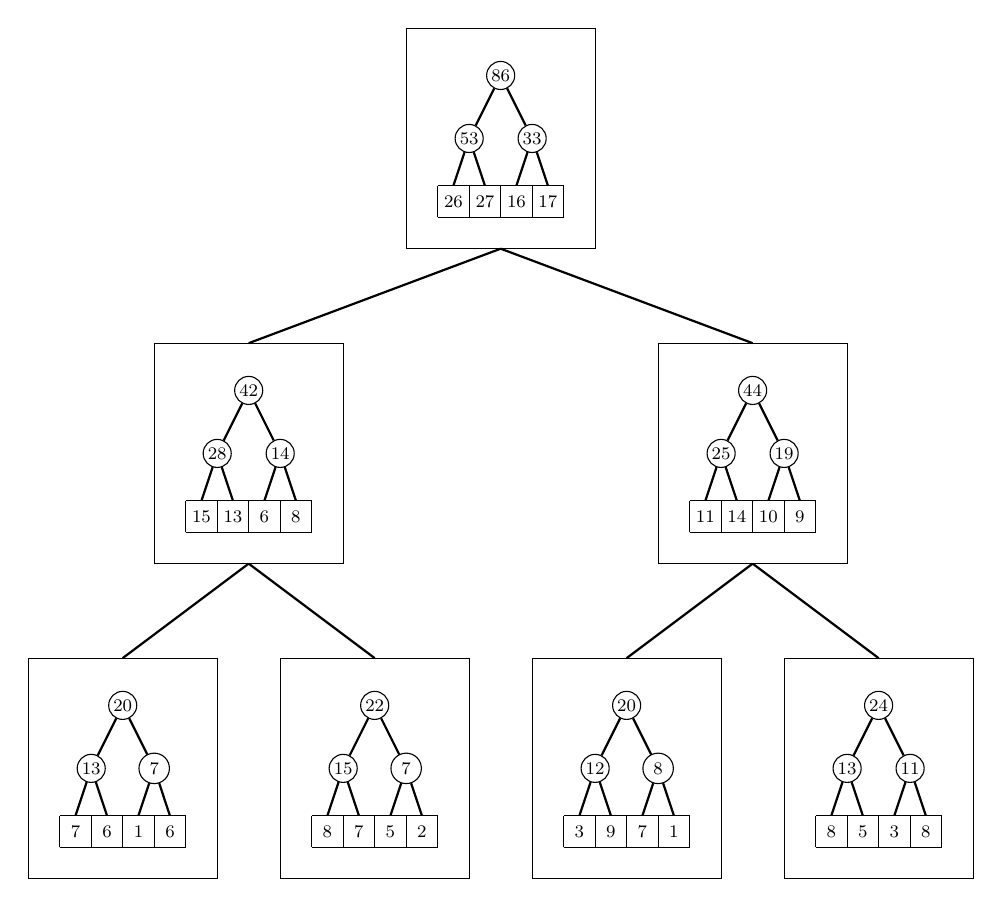
\begin{tikzpicture}[scale=0.4]
\footnotesize
\begin{scope}[shift={(-12,0)}]
\draw (-1,-1) rectangle (5,6);
\draw (0,0) grid (4,1);
\node[anchor=center,scale=0.8] at (0.5, 0.5) {7};
\node[anchor=center,scale=0.8] at (1.5, 0.5) {6};
\node[anchor=center,scale=0.8] at (2.5, 0.5) {1};
\node[anchor=center,scale=0.8] at (3.5, 0.5) {6};

\node[draw, circle,scale=0.8,inner sep=1pt] (a) at (1,2.5) {13};
\path[draw,thick,-] (a) -- (0.5,1);
\path[draw,thick,-] (a) -- (1.5,1);
\node[draw, circle,scale=0.8,inner sep=2.5pt] (b) at (3,2.5) {7};
\path[draw,thick,-] (b) -- (2.5,1);
\path[draw,thick,-] (b) -- (3.5,1);

\node[draw, circle,scale=0.8,inner sep=1pt] (i) at (2,4.5) {20};
\path[draw,thick,-] (i) -- (a);
\path[draw,thick,-] (i) -- (b);
\end{scope}
\begin{scope}[shift={(-4,0)}]
\draw (-1,-1) rectangle (5,6);
\draw (0,0) grid (4,1);
\node[anchor=center,scale=0.8] at (0.5, 0.5) {8};
\node[anchor=center,scale=0.8] at (1.5, 0.5) {7};
\node[anchor=center,scale=0.8] at (2.5, 0.5) {5};
\node[anchor=center,scale=0.8] at (3.5, 0.5) {2};

\node[draw, circle,scale=0.8,inner sep=1pt] (a) at (1,2.5) {15};
\path[draw,thick,-] (a) -- (0.5,1);
\path[draw,thick,-] (a) -- (1.5,1);
\node[draw, circle,scale=0.8,inner sep=2.5pt] (b) at (3,2.5) {7};
\path[draw,thick,-] (b) -- (2.5,1);
\path[draw,thick,-] (b) -- (3.5,1);

\node[draw, circle,scale=0.8,inner sep=1pt] (i) at (2,4.5) {22};
\path[draw,thick,-] (i) -- (a);
\path[draw,thick,-] (i) -- (b);
\end{scope}
\begin{scope}[shift={(4,0)}]
\draw (-1,-1) rectangle (5,6);
\draw (0,0) grid (4,1);
\node[anchor=center,scale=0.8] at (0.5, 0.5) {3};
\node[anchor=center,scale=0.8] at (1.5, 0.5) {9};
\node[anchor=center,scale=0.8] at (2.5, 0.5) {7};
\node[anchor=center,scale=0.8] at (3.5, 0.5) {1};

\node[draw, circle,scale=0.8,inner sep=1pt] (a) at (1,2.5) {12};
\path[draw,thick,-] (a) -- (0.5,1);
\path[draw,thick,-] (a) -- (1.5,1);
\node[draw, circle,scale=0.8,inner sep=2.5pt] (b) at (3,2.5) {8};
\path[draw,thick,-] (b) -- (2.5,1);
\path[draw,thick,-] (b) -- (3.5,1);

\node[draw, circle,scale=0.8,inner sep=1pt] (i) at (2,4.5) {20};
\path[draw,thick,-] (i) -- (a);
\path[draw,thick,-] (i) -- (b);
\end{scope}
\begin{scope}[shift={(12,0)}]
\draw (-1,-1) rectangle (5,6);
\draw (0,0) grid (4,1);
\node[anchor=center,scale=0.8] at (0.5, 0.5) {8};
\node[anchor=center,scale=0.8] at (1.5, 0.5) {5};
\node[anchor=center,scale=0.8] at (2.5, 0.5) {3};
\node[anchor=center,scale=0.8] at (3.5, 0.5) {8};

\node[draw, circle,scale=0.8,inner sep=1pt] (a) at (1,2.5) {13};
\path[draw,thick,-] (a) -- (0.5,1);
\path[draw,thick,-] (a) -- (1.5,1);
\node[draw, circle,scale=0.8,inner sep=1pt] (b) at (3,2.5) {11};
\path[draw,thick,-] (b) -- (2.5,1);
\path[draw,thick,-] (b) -- (3.5,1);

\node[draw, circle,scale=0.8,inner sep=1pt] (i) at (2,4.5) {24};
\path[draw,thick,-] (i) -- (a);
\path[draw,thick,-] (i) -- (b);
\end{scope}
\begin{scope}[shift={(-8,10)}]
\draw (-1,-1) rectangle (5,6);
\draw (0,0) grid (4,1);
\node[anchor=center,scale=0.8] at (0.5, 0.5) {15};
\node[anchor=center,scale=0.8] at (1.5, 0.5) {13};
\node[anchor=center,scale=0.8] at (2.5, 0.5) {6};
\node[anchor=center,scale=0.8] at (3.5, 0.5) {8};

\node[draw, circle,scale=0.8,inner sep=1pt] (a) at (1,2.5) {28};
\path[draw,thick,-] (a) -- (0.5,1);
\path[draw,thick,-] (a) -- (1.5,1);
\node[draw, circle,scale=0.8,inner sep=1pt] (b) at (3,2.5) {14};
\path[draw,thick,-] (b) -- (2.5,1);
\path[draw,thick,-] (b) -- (3.5,1);

\node[draw, circle,scale=0.8,inner sep=1pt] (i) at (2,4.5) {42};
\path[draw,thick,-] (i) -- (a);
\path[draw,thick,-] (i) -- (b);
\end{scope}
\begin{scope}[shift={(8,10)}]
\draw (-1,-1) rectangle (5,6);
\draw (0,0) grid (4,1);
\node[anchor=center,scale=0.8] at (0.5, 0.5) {11};
\node[anchor=center,scale=0.8] at (1.5, 0.5) {14};
\node[anchor=center,scale=0.8] at (2.5, 0.5) {10};
\node[anchor=center,scale=0.8] at (3.5, 0.5) {9};

\node[draw, circle,scale=0.8,inner sep=1pt] (a) at (1,2.5) {25};
\path[draw,thick,-] (a) -- (0.5,1);
\path[draw,thick,-] (a) -- (1.5,1);
\node[draw, circle,scale=0.8,inner sep=1pt] (b) at (3,2.5) {19};
\path[draw,thick,-] (b) -- (2.5,1);
\path[draw,thick,-] (b) -- (3.5,1);

\node[draw, circle,scale=0.8,inner sep=1pt] (i) at (2,4.5) {44};
\path[draw,thick,-] (i) -- (a);
\path[draw,thick,-] (i) -- (b);
\end{scope}
\begin{scope}[shift={(0,20)}]
\draw (-1,-1) rectangle (5,6);
\draw (0,0) grid (4,1);
\node[anchor=center,scale=0.8] at (0.5, 0.5) {26};
\node[anchor=center,scale=0.8] at (1.5, 0.5) {27};
\node[anchor=center,scale=0.8] at (2.5, 0.5) {16};
\node[anchor=center,scale=0.8] at (3.5, 0.5) {17};

\node[draw, circle,scale=0.8,inner sep=1pt] (a) at (1,2.5) {53};
\path[draw,thick,-] (a) -- (0.5,1);
\path[draw,thick,-] (a) -- (1.5,1);
\node[draw, circle,scale=0.8,inner sep=1pt] (b) at (3,2.5) {33};
\path[draw,thick,-] (b) -- (2.5,1);
\path[draw,thick,-] (b) -- (3.5,1);

\node[draw, circle,scale=0.8,inner sep=1pt] (i) at (2,4.5) {86};
\path[draw,thick,-] (i) -- (a);
\path[draw,thick,-] (i) -- (b);
\end{scope}
\path[draw,thick,-] (2,19) -- (-6,16);
\path[draw,thick,-] (2,19) -- (10,16);
\path[draw,thick,-] (-6,9) -- (-10,6);
\path[draw,thick,-] (-6,9) -- (-2,6);
\path[draw,thick,-] (10,9) -- (6,6);
\path[draw,thick,-] (10,9) -- (14,6);
\end{tikzpicture}
\end{center}

The operations of a two-dimensional segment tree
take $O(\log^2 n)$ time, because the big tree
and each small tree consist of $O(\log n)$ levels.
The tree requires $O(n^2)$ memory, because each
small tree contains $O(n)$ values.
